%dus was ik aan het nadenken over de stand van zaken na dynbenchmark ─ oké, ik heb zin om een dynbenchmark2 te doen moet, alles meer en beter
%maar hoe hebben we een impact gehad? als je kijkt naar course material over trajectory inference zou ik zeggen, veel ─ we zijn een gemakkelijke bron van guidelines
%maar als ik kijk naar de manuscripten van nieuwe TI methoden zou ik zeggen dat we nog niet zijn waar we wouden geraken

\section{Self-assessment in trajectory inference}
Many trajectory inference (TI) tools lack quantitative assessment of the accuracy of the method. Instead, they rely on anecdotal evidence to demonstrate their added value. A brief review of 75 TI articles reveals that only about 37\% contain a self-assessment (Figure \ref{fig:benchmarks_over_time}). Peer-reviewed TI articles fared even worse, self-assessing in only 34\% of cases (n=55), whereas articles first published as a pre-print self-assess in 43\% of cases (n=39). Only three TI articles feature a comparison of at least 5 methods using 5 datasets or more \cite{sharma_forksfindingorderings_2017,guo_hoplandsinglecellpseudotime_2017,parra_reconstructingcomplexlineage_2018}.

Self-assessments are universally biased in favour of the authors, intentionally or otherwise, but this does not mean they should be skipped out on. Norel et al. provide a valuable discussion on overcoming overly optimistic self-assessments \cite{norel_selfassessmenttrapcan_2011}.
% TODO: improve working "this does not mean they should be skipped out on"

In this perspective, we hypothesise that low self-assessment rates are primarily caused by a lack of a standardised problem definition, benchmarking datasets, and metrics. 
We elaborate on these reasons and viable solutions to easy benchmarking trajectory inference.

\begin{figure}[htb!]
	\centering
	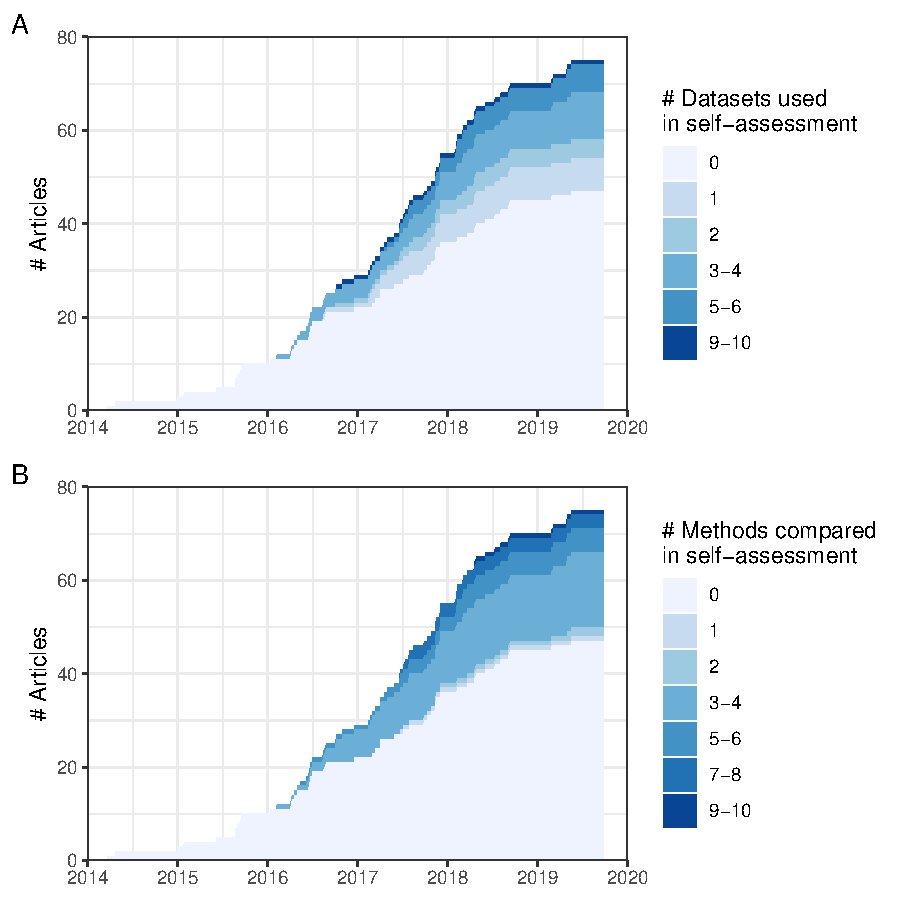
\includegraphics[width=.75\linewidth]{fig/self_assessment.pdf} 
	\caption{\textbf{The number of manuscripts featuring trajectory inference tools over time.} Areas coloured in darker shades of blue represent manuscripts containing self-assessment of the tool, highlighting \textbf{A}: the number of datasets used and \textbf{B}: the number of methods used (including the method of the authors).}
	\label{fig:benchmarks_over_time}
\end{figure}

\subsection{Problem definition}
One main reason why benchmarking TI methods is difficult is due to there being slight variations 
of the problem a method is attempting to solve (Figure \ref{fig:method_types}A). For example, a method might infer linear or cyclic trajectories, or predict the probability of a cell ending up in one of several end states.

\begin{figure}[htb!]
	\centering
	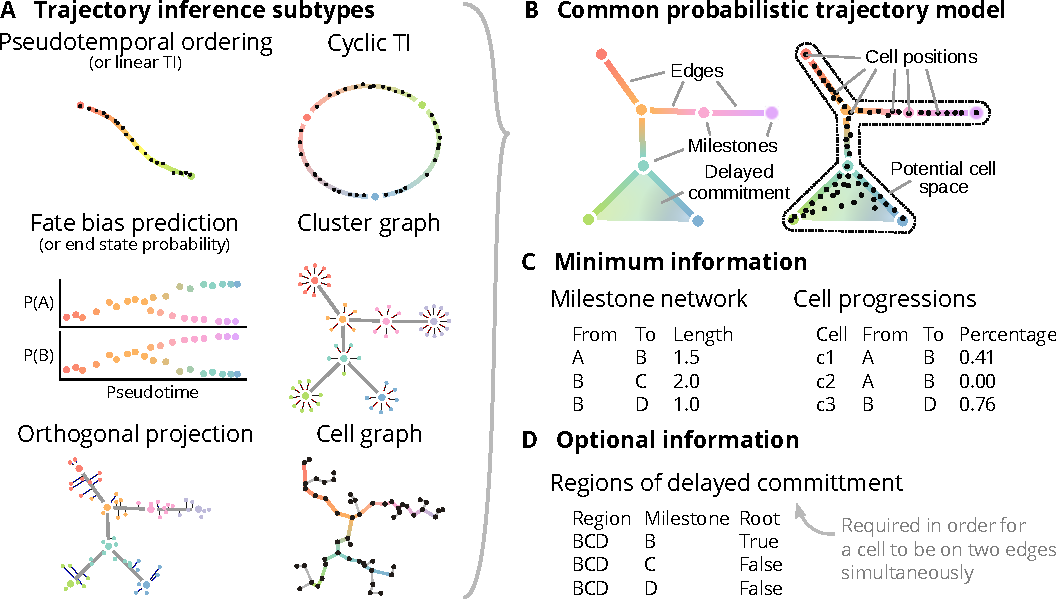
\includegraphics[width=\linewidth]{fig/method_types.pdf} 
	\caption{
		\textbf{Different forms of trajectory inference.}
		\textbf{A:} All TI methods can be categorised in one of seven subtypes in terms of its produced output \cite{saelens_comparisonsinglecelltrajectory_2019}.
		\textbf{B:} Each of these can be translated into a common format, allowing easier comparison of multiple trajectories.
		\textbf{C:} The minimum information required to describe a trajectory in this way is the milestone network -- representing transitions between cellular states -- and the cell progressions -- representing the positions of cells along the transitions.
		\textbf{D:} Optionally, regions of delayed commitment can be defined. A region of delayed commitment contain multiple transitions starting from the same milestone. This allows a TI method to assign probabilities on how likely a cell is part of one of these transitions.
	}
	\label{fig:method_types}
\end{figure}

As a result, it becomes harder to discover similar methods to compare against, as certain articles might only show up with search terms such as "pseudotemporal ordering", "lineage trees" or "fate bias". For the discoverability of a new TI method, it is therefore essential to use the term "trajectory inference", or at least list it as one of the keywords. 

A more significant and harder to solve problem is that the data formats produced by different methods varies greatly. This makes visualising and comparing multiple trajectories difficult, as different output types cannot be compared directly. The most commonly used and general is one where cells are positioned along a set of edges connecting milestones ("Regular TI", Figure~\ref{fig:method_types}A). 
By adding an extension to regular TI to allow for cells to be part of three or more cellular states, thereby a cell to delay its commitment toward a particular end state (Figure~\ref{fig:method_types}B). 

By adding this extension, all TI subtypes can easily be converted into the common format. Implementations of these conversions can be found in \texttt{dynwrap}\cite{dyno}. Using this standardised format allows developing reusable software for visualising and comparing trajectories from different TI methods.

In practice, this format consists of two data structures: the milestone network specify transition between cell states, and the cell progressions specify how far along each cell has progressed along a transition (Figure~\ref{fig:method_types}C). In addition, regions of delayed commitment need to be specified, if any (Figure~\ref{fig:method_types}D). 

\mycomment{examples? elaborate? citation?}

\subsection{Benchmarking datasets}
Another hurdle in benchmarking trajectory inference methods is collecting datasets to benchmark against. Before 2018, there were only a handful of datasets containing complex trajectories (Figure~\ref{fig:datasets}). 

When real data is scarce, synthetic data is often used to evaluate computational methods, either standalone (n=5) or to complement real data (n=7). Most synthetic data is generated by the authors themselves (n=8), whereas some reuse datasets generated by others (n=3) or use one of the readily available simulators (n=2). To avoid introducing self-assessment bias in a benchmark, it is recommended to use readily available simulators if they fit the requirements. Examples are dyntoy \cite{saelens_comparisonsinglecelltrajectory_2019}, dyngen \cite{dyngen}, splatter \cite{zappia_splattersimulationsinglecell_2017}, and PROSSTT \cite{papadopoulos_prossttprobabilisticsimulation_2018}.

Benefits of synthetic data are that they offer more control over the data characteristics, and that they can be generated in large quantities. This allows to evaluate performance of a method in function of a changing parameter (e.g. dataset size or noise levels), which provides information on how well the method will work on real datasets.

A common counterargument of synthetic data is that they generate unrealistic datasets and thus provide no additional value in evaluation a method. In contrast, we argue that a good set of synthetic datasets should allow benchmarkers to verify that a method should \textit{at least} work well on the synthetic datasets, but good performance on synthetic datasets does not guarantee good performance on real datasets.

Several authors use mainly real datasets to evaluate their method, though only few use more than four datasets (n=7). 
By now, already hundreds of suitable real datasets exist (Figure~\ref{fig:datasets}). Downloading and pre-processing them requires a significant time investment, but by processing the datasets once and storing them in a single repository they can be reused for multiple purposes.

Readers are welcome to reuse (and extend) the 110 real and 229 synthetic datasets used in our comparison of TI methods. The datasets are hosted on Zenodo\cite{cannoodt_singlecellomicsdatasets_2018} and the scripts to process them on GitHub\footnote{\href{https://github.com/dynverse/dynbenchmark/tree/master/scripts/01-datasets}{github.com/dynverse/dynbenchmark/tree/master/scripts/01-datasets}}. Note that the ground truths of the datasets are represented using the common data structures format in the previous section.

\begin{figure}[htb!]
	\centering
	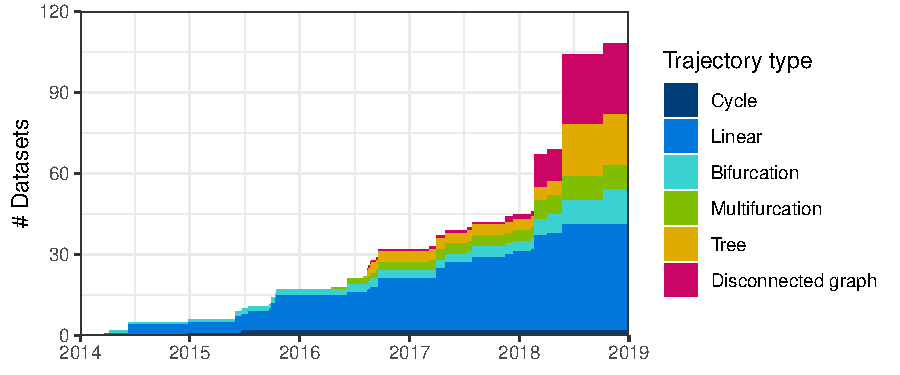
\includegraphics[width=.75\linewidth]{fig/datasets.pdf} 
	\caption{\textbf{An overview collection of TI benchmarking datasets in function of their publication date and the topology of the trajectory.} These datasets are readily available on Zenodo\cite{cannoodt_singlecellomicsdatasets_2018}.}
	\label{fig:datasets}
\end{figure}


\subsection{Multiple metrics}


%in deze commentary geven we nog een kort overzicht van:
%* standaard definitie van een trajectory inference probleem
%* waar kan je datasets vinden (dynbenchmark zenodo, de verschillende simulatoren, of download ze zelf van GEO)
%* hoe kan je methoden vergelijken (i.e. gebruik dynmethods)
%* wat zijn bestaande metrieken (toon overzicht van metrieken uit verschillende benchmarks en ook die van dyneval)
%in conclusie, met al deze informatie melden we dat in 2019 er dus geen enkele reden is om ons te gedragen als gelijk welk ander computationeel / data mining / machine learning veld waarbij er voor quantitatief bewijs wordt gevraagd dat je methode goed werkt als je een nieuwe methode wilt publiceren. we vragen vriendelijk aan peer-reviewers om kritisch te zijn over deze kwestie.

%in deze commentary geven we nog een kort overzicht van:
%* standaard definitie van een trajectory inference probleem
%* waar kan je datasets vinden (dynbenchmark zenodo, de verschillende simulatoren, of download ze zelf van GEO)
%* hoe kan je methoden vergelijken (i.e. gebruik dynmethods)
%* wat zijn bestaande metrieken (toon overzicht van metrieken uit verschillende benchmarks en ook die van dyneval)

%in conclusie, met al deze informatie melden we dat in 2019 er dus geen enkele reden is om ons te gedragen als gelijk welk ander computationeel / data mining / machine learning veld waarbij er voor quantitatief bewijs wordt gevraagd dat je methode goed werkt als je een nieuwe methode wilt publiceren. we vragen vriendelijk aan peer-reviewers om kritisch te zijn over deze kwestie.

%refer to: \cite{norel_selfassessmenttrapcan_2011} 
%In order to alleviate the overestimation of accuracy from the many bias sources described above, we proposed a few guidelines:
%* use third‐party validation to test a model with previously unseen data
%* use more than one metric to evaluate the methods
%* report well‐performing methods even if they are not the best performers on a particular data set
%* increase the awareness of editors and reviewers that superior performance in self‐assessment is a biased demonstration of the method's value; instead, impartial assessment should be the preferred evaluation
%* Establish a scientific culture that values timely, well‐conducted follow‐up studies that confirm or refute previous results




%Before 2016, only a handful of trajectory inference methods had been released. None of these articles contained a self-benchmark simply because
%
%In all fairness towards the early TI methods, in 2016 or even 2017 there was a low abundance of good datasets to perform benchmarks with. The amount of data required to perform a comprehensive evaluation of their tool did not yet exist and was too expensive to generate. In April 2016, we started developing a single-cell simulator that would allow us to perform a comprehensive benchmark of TI methods. 
%
%
%It was also non-trivial to compare against many methods as each method has a unique interface where some prior knowledge might be needed. 
%


% * Single cell omics is expanding at rates faster than any single mind can try to conceive
%Pioneers developing revolutionary tools to process new types of data are typically faced with the problem on how to quantitatively evaluate the accuracy of their approach. After all, the amount of data required to perform a comprehensive evaluation of their tool does not yet exist and is too expensive to generate at the time. 


%In the computational jungle of single-cell omics, experts act as beacons of hope by sharing guidelines based on comprehensive benchmarking studies. Their disseminations (in the form of manuscripts \cite{lafzi_tutorialguidelinesexperimental_2018,luecken_currentbestpractices_2019}, courses \cite{kiselev_analysissinglecell_2019,martens_analysissinglecell_2019}, and slides shown during keynote caffeine refuelling sessions \cite{hemberg_coffeebreakanalysis_2019}) are crucial in leading new users, and ultimately the whole field, to better practices for performing single-cell omics analyses.

%Before embarking on this perilous adventure, I attempt to write a "Hippocratic oath for bioinformaticians", to guide me through this dissertation and not stray from the path of righteousness.
%
%\subsection{Hippocratic oath for bioinformaticians}
%We proceed with caution in developing new tools. Its results should not only be convincing and easy to interpret, but also accurate, robust, and reproducible. We open source. Our software should work reliably and fail gracefully when it does not. We acknowledge that writing automated tests is dull but necessary for maintaining long-term software projects. % TODO: improve

%Computer scientists should proceed with caution in developing new software, however, as the results produced should not only be convincing and easy to interpret, but the software should be robust and generate sufficiently accurate models of the underlying system.
%
%Bit too excited -- false positives, poor accuracy, scalability issues, poor software quality. 

\section{dyngen discussion}
% felt that upon the development of a new technologies, good quality control practices from
% other technologies were not being carried over because the data required to evaluate computational
% tools does not exist yet and is too expensive to develop.

\section{dynbenchmark discussion}
\begin{itemize}
	\item Already outdated when the manuscript was published online
	\item Update benchmark with more TI methods, newer (and larger) datasets, perform parameter optimisation on methods
	\item Include RNA velocity as inputs
\end{itemize}

\section{SCORPIUS discussion}
\begin{itemize}
	\item Extension to inferring non-linear trajectories, i.e. with principal graphs
\end{itemize}

\section{bred discussion}

%\section{incgraph discussion}

%\section{dyno discussion}

